\outlineSubframe{Formale Eigenschaften}

\begin{frame}{Eigenschaften von Algorithmen}{Grundlegendes}
    \begin{itemize}[<+->]
        \item \textbf{Finitheit} - Ein Algorithmus lässt sich in endlch vielen Schritten eindeutig beschreiben
        \item \textbf{Ausführbarkeit} - Jeder Einzelschritt muss tatsächlich ausführbar sein
        \item \textbf{Platzkomplexität} - Ein Algorithmus benötigt zu jedem Zeitpunkt nur endlich viel Speicherplatz
        \item \textbf{Terminierung} - Der Algorithmus benötigt eine endliche Anzahl von Schritten zur Ausführung
        \item \textbf{Determiniertheit} - Der Algorithmus muss bei gleichen Rahmenbedingungen das gleiche Ergebnis liefern
        \item \textbf{Determinismus} - Der nächste Schritt des Algorithmus ist zu jedem Zeitpunkt genau definiert
    \end{itemize}
\end{frame}

\begin{frame}{Korrektheit von Algorithmen}{}
    \begin{itemize}[<+->]
        \item Jeder Algorithmus sollte auch in allen Fällen das korrekte Ergebnis liefern...
        \item Klingt simpel, aber eindeutiger Beweis für alle Eingaben oft schwierig
        \item Testen an ausgewählten Beispielen \textbf{nicht} ausreichend
        \begin{itemize}
            \item Jedoch verringern umfangreiche Tests natürlich das Risiko eines unentdeckten Fehler
        \end{itemize}
        \item Korrektheit lässt sich im Grunde nur durch formalen Beweis zeigen
        \begin{itemize}
            \item Diese sind häufig sehr umfangreich und komplex...
            \item ...und deshalb auch nicht Teil der Vorlesung
        \end{itemize}
    \end{itemize}
\end{frame}

\begin{frame}{Korrektheit von Algorithmen}{}
\begin{minipage}{0.4\textwidth}
            \begin{figure}
                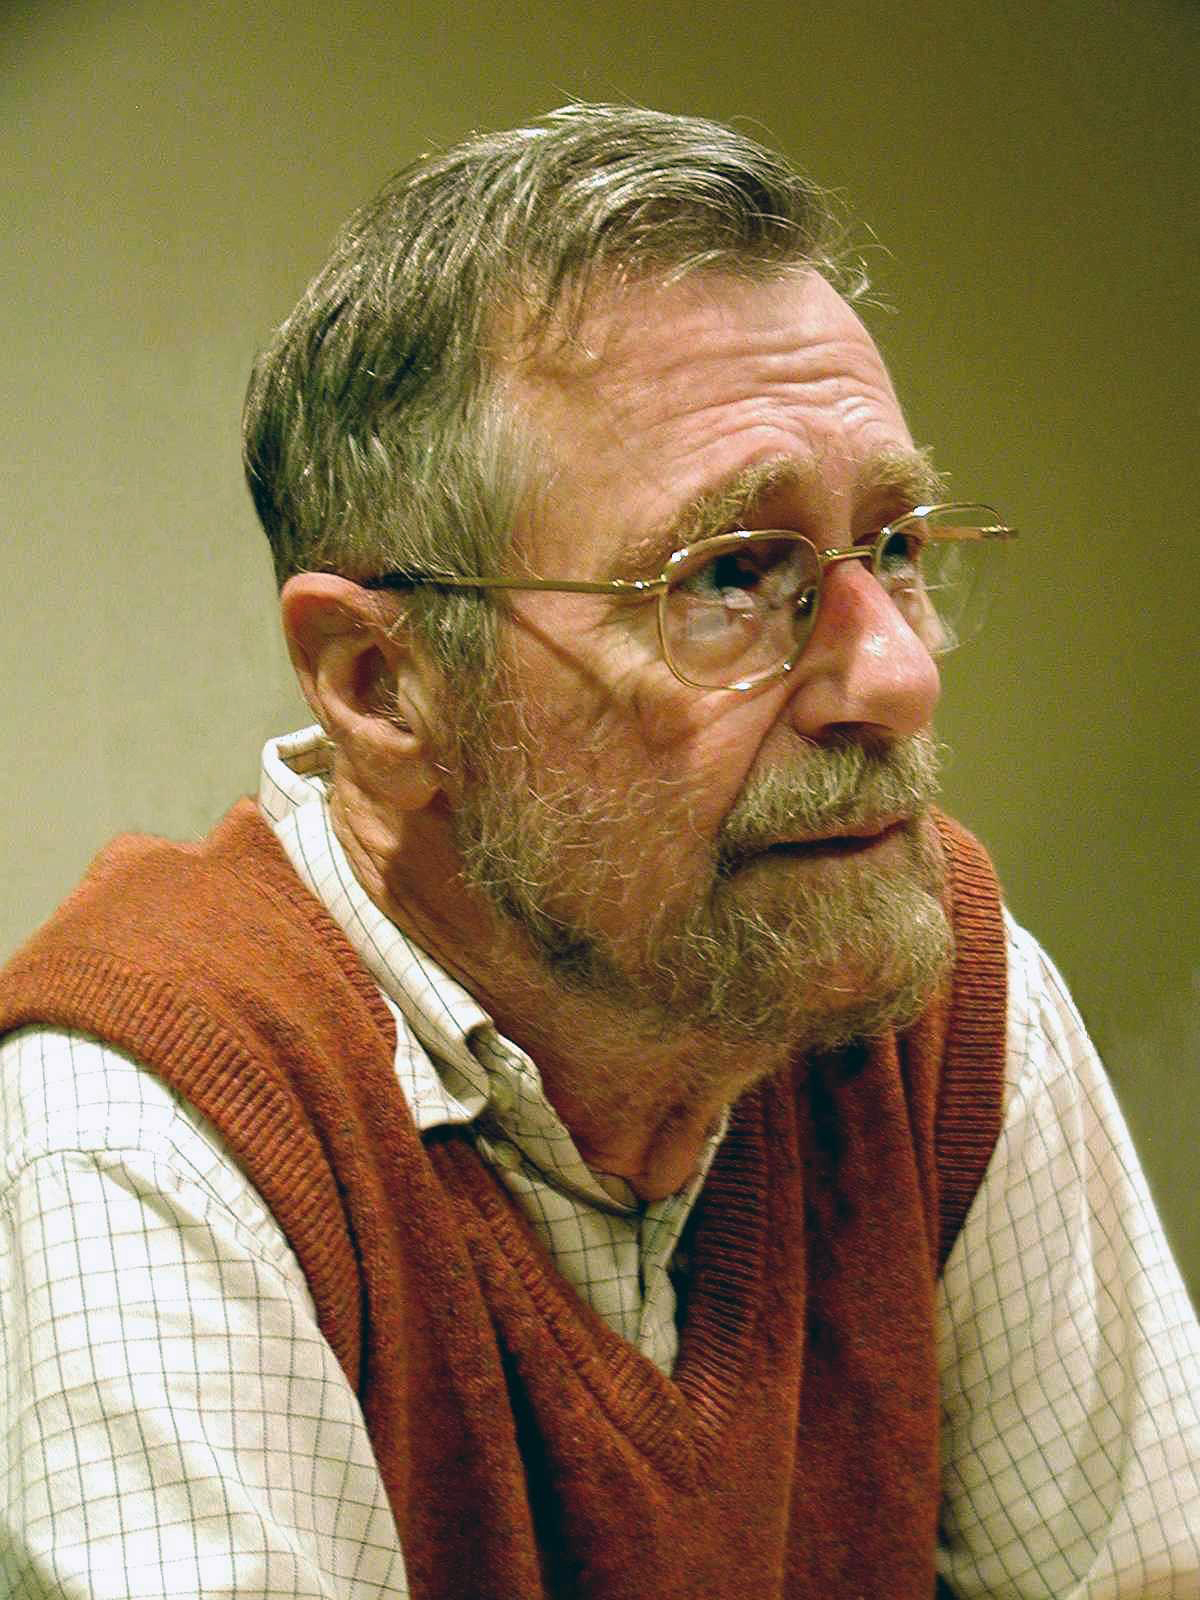
\includegraphics[height=4.5cm]{graph/dijkstra}
                \caption*{Quelle: }%\url{https://upload.wikimedia.org/wikipedia/commons/d/d9/Edsger_Wybe_Dijkstra.jpg}}
            \end{figure}
        \end{minipage}
        \hfill
        \begin{minipage}{0.55\textwidth}
            \textit{„Program testing can be used to show the presence of bugs, but never to show their absence!.“} \\\\Edsger W. Dijkstra
        \end{minipage}
\end{frame}

\begin{frame}{Effizienz von Algorithmen}{}
    \begin{itemize}
        \item Ergibt sich indirekt aus den Grundlegenden Eigenschaften
        \item Effizienz lässt sich über verschiedene Größen beschreiben:
        \begin{itemize}
            \item Speicherverbrauch
            \item Zeitverbrauch
        \end{itemize}
        \item Die sind jedoch oft Implementierungs- und Rechnerabhägig
        \item Deshalb wird mit formalisierten Modellen gearbeitet
        \item ...Mehr dazu im Kapitel "`Analyse"'
    \end{itemize}
\end{frame}

\outlineSubframe{Darstellungsformen}

\begin{frame}{}
\end{frame}